\chapter{Komplexe Zahlen}


\section{Einführung}

	\paragraph{} Die Ursache für die Einführung der komplexen Zahlen ist vergleichbar mit der jeglicher anderer Zahlenmengen (abgesehen
	von $\N$). Alles basiert auf einer Rechnung oder einer Menge an Rechnungen, welche für die vorhandenen Zahlenmengen \textbf{keine Lösung
	besitzen} oder aber diese Zahlenmengen einem nicht erlauben eine Lösung zu finden. Ein Beispiel hierfür ist die Einführung der
	negativen Zahlen. Gleichungen der Form $2 + x = 1$ waren eine Zeit lang nicht lösbar. Ebenso galt einmal, dass $x^2 - 2 = 0$ keine
	Lösung besitzt, da hierfür die reellen Zahlen benötigt werden. Analog dazu wird die Erweiterung auf die komplexen Zahlen begründet.
	Dies wird an folgendem klassischen Beispiel erläutert:

	\begin{align*}
		\qquad \qquad x^2 + 1 &= 0 \\
			\Leftrightarrow x &= \sqrt{-1} \quad \text{\Lightning}
	\end{align*}

	\paragraph{} Um dieser und anderen Gleichungen eine Lösung zuzuteilen ist es nicht nur notwendig die Zahlenmenge zu erweitern, sondern
	auch, neue Symbole und Zeichen einzuführen um die neuen Zahlen zu kennzeichnen. Für die $\Z$ ist es das Symbol \dq-\dq, für $\Q$
	\dq,\dq und $\dfrac{a}{b}$, für $\R$ $\sqrt{a}$ und die Zeichen $\pi$ und $e$ zum Beispiel (auch wenn beide sich anders darstellen lassen).
	(Ein) gewisse(r) Mathematiker (Leibniz glaube ich) hat entschieden, dass das einzige benötigte Zeichen $i$ sein sollte, da er sie imaginäre
	Zahl nannte (Für den Fall, dass ich hier ein bisschen was durcheinander bringe, sind Direktverbesserungen kommentarlos erlaubt und erwünscht).
 	Und dem war so, weshalb nun gilt:
											$$i \in \C : i^2 = -1; \C \definedBy \R \cup \right\text\{i\left\}$$

	\begin{Definition}
		Komplexe Zahlen werden standartmäßig mit dem Buchstaben $z$ dargestellt. Die allgemeine Formel einer solchen Zahl lautet:
		\\
		\begin{tikzpicture}
			\draw (0,0) node {};
			\draw (7.9, 0) node {$z = x + y \cdot i; x,y \in \R; i \in \C$};
			\draw[line width=0.8pt][decorate,decoration={brace,amplitude=3pt},rotate around={180:(7.6,-0.25)}] (7.6,-0.25) -- (8.1,-0.25);
			\draw[line width=0.8pt][decorate,decoration={brace,amplitude=2pt},rotate around={180:(6.7,-0.25)}] (6.7,-0.25) -- (7,-0.25);
		    \draw[line width=0.4pt] (6.55,-0.5) -- (5.1,-1.4) node[color=blue,left] {$Re(z)$};
		    \draw[line width=0.4pt] (7.35,-0.5) -- (9.2,-1.4) node[color=blue,right] {$Im(z)$};
		\end{tikzpicture}
		\\
		Hierbei wird $x = Re(z)$ Realteil und $y = Im(z)$ und zwar \bold{nur $y$} Imaginärteil genannt.
	\end{Definition}

	\begin{Bemerkung}
		Eine Zahl $z = x + yi \in \C$ heißt rein imaginäre Zahl für $x = 0$. Analog dazu wird sie für $y = 0$ als reell bezeichnet.
	\end{Bemerkung}


\section{Der Körper der komplexen Zahlen}

	\paragraph{} Da wir nun wissen (oder halt auch nicht), weshalb wir die komplexen Zahlen benötigen, gilt es nun die verschiedenen Verknüpfungen,
	mit welchen wir zwei komplexe Zahlen verbinden, zu definieren. Wie alle anderen bekannten Mengen (außer $\N$), ist $\C$ teil eines \textbf{Körpers}
	welcher die zwei Verknüpfungen, denen wir allgemein die Namen \textbf{Addition} und \textbf{Multiplikation} geben. Das 3-Tupel (oder auch Tripel)
	($\C$, +, *) ist somit der Körper, mit welchem wir arbeiten werden (jemals gefragt warum keine weiteren Verknüpfungen eingeführt wurden?).
	Jedoch muss auch erstmal bewiesen werden, dass dieses Tripel ein Körper ist:

	\begin{Beweis}
		\underline{\textbf{Die Addition}}:

		\paragraph{} Für die Addition gilt bekanntlich zu beweisen, dass ($\C$, \oplus) eine abelsche oder auch kommutative Gruppe ist:

		\begin{enumerate}[1)]
			\item \begin{align*}
						\forall z_1, z_2 \in \C: z_1 \oplus z_2 &\definedBy (x_1 + y_1i) \oplus (x_2 + y_2i) \\
														   		&= ((x_1 + x_2) + (y_1 + y_2)i) \\
														   		&\in \C \\
						\Rightarrow \forall z_1, z_2 \in \C: \oplus : \C \times \C \rightarrow \C \quad \text{(Abges}&\text{chlossenheit)}
				  \end{align*}
			\item \begin{align*}
				  		(z_1 \oplus z_2) \oplus z_3 &= ((x_1 + x_2) + (y_1 + y_2)i) \oplus (x_3 + y_3i) \\
										  			&= ((x_1 + x_2 + x_3) + (y_1 + y_2 + y_3)i) \\
												    &= (x_1 + y_1i) \oplus ((x_2 + x_3) + (y_2 + y_3)i) \\
												    &= (x_1 + y_1i) \oplus ((x_2 + y_2i) \oplus (x_3 + y_3i)) \\
												    &= z_1 \oplus (z_2 \oplus z_3) \\
						\Rightarrow \forall z_1, z_2, z_3 \in \C: &(z_1 + z_2) \oplus z_3 = z_1 \oplus (z_2 + z_3) \quad \text{(Assoziativität)}
				  \end{align*}
			\item \begin{align*}
						e = (0 + 0i) \in \C, z \in \C: z \oplus e &= (x + yi) \oplus (0 + 0i) \\
															 	  &= ((x + 0) + (y + 0)i) \\
															 	  &= (x + yi) \\
						\Rightarrow \exists e : z \oplus e = z; z \in \C \quad \text{(Neutrales Element)}&
				  \end{align*}
			%\item \begin{align*}
	  		%			z* = (0 + 0i) \in \C, z \in \C: z \oplus e &= (x + yi) \oplus (0 + 0i) \\
	  		%												 	  &= ((x + 0) + (y + 0)i) \\
	  		%													  &= (x + yi) \\
	  		%			\Rightarrow \exists e : z \oplus e = z; z \in \C \quad \text{(Neutrales Element)}&
	  		%		  \end{align*}
			\item \begin{align*}
						z_1 \oplus z_2 &= (x_1 + y_1i) \oplus (x_2 + y_2i) \\
									   &= ((x_1 + x_2) + (y_1 + y_2)i) \\
									   &= ((x_2 + x_1) + (y_2 + y_1)i) \\
									   &= (x_2 + y_2i) \oplus (x_1 + y_1i) \\
									   &= z_2 \oplus z_1 \\
						\Rightarrow \forall z_1, z_2 \in \C: z_1 \oplus z_2 = z_2 \oplus z_1 \quad \text{(Kom}&\text{mutativität)}
				  \end{align*}
		\end{enumerate}
	\end{Beweis}

\section{Darstellung komplexer Zahlen}

	Eine komplexe Zahl wird durch zwei reelle Zahlen charakterisiert. Wie bei zweidimensionalen Vektoren brauchen wir hier zur geometrischen Veranschaulichung auch eine zweidimensionale Ebene.\\

	\subsection{Kartesische Darstellung}

		Jeder komplexen Zahl $z =x+i*y$ entspricht genau ein Punkt $P =(x,y)$ in der komplexen Zahlenebene und umgekehrt.\\

		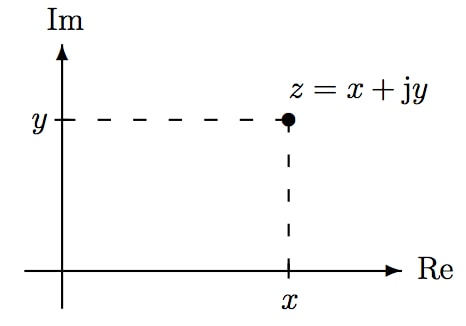
\includegraphics[width=3in]{kap6/komplexezahlen1}

		\begin{Bemerkung}
		Bezeichnungen\\
		\end{Bemerkung}

		\begin{enumerate}
		\item Die komplexe Zahlenebene nennt sich auch Gaußsche- Zahlenebene
		\item Hier werden die Achsen des Koordinatensystems als \textbf{reelle Achse} bzw. \textbf{imagin"are Achse} bezeichnet.\\
		\end{enumerate}

		\begin{Bemerkung}
		Beispiel\\
		\end{Bemerkung}

		Die folgenden komplexen Zahlen sind in der Gaußschen Zahlenebene darzustellen: \\
		$z_{1} = 2+3*j$  $z_{2} =-3-j$ ($i$ wird hier $j$ genannt)

		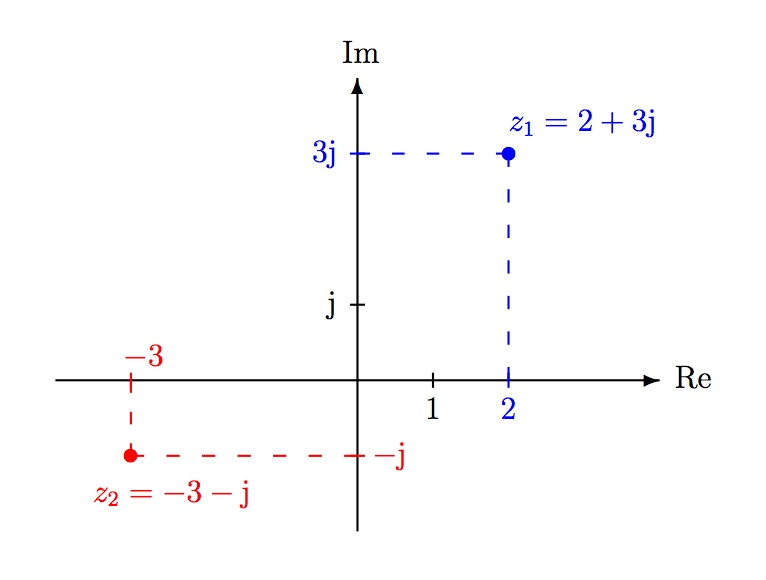
\includegraphics[width=3in]{kap6/komplexezahlen2}

		\begin{Bemerkung}
		Bemerkungen\\
		\end{Bemerkung}

		F"ur manche Anwendungen ist es hilfreich, eine komplexe Zahl nicht als Punkt $P=(x,y)$ in der Gaußschen Zahlenebene zu veranschaulichen, sondern stattdessen den Ortsvektor zu betrachten

		$z=x+j*y \Leftrightarrow z=
		\begin{pmatrix}
		x\\
		y\\
		\end{pmatrix}$

		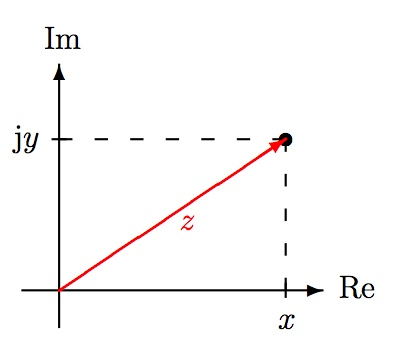
\includegraphics[width=3in]{kap6/komplexezahlen3}

		In diesem Fall spricht man von z als einem \textbf{komplexen Zeiger}.\\

	\subsection{Polarkoordinatendarstellung}

		Neben der eben eingef"uhrten kartesischen Darstellung $z =x+j*y$ kann eine komplexe Zahl auch entsprechend der hier stehenden Skizze dich ihren Radius  und den Winkel  eindeutig festgelegt werden.

		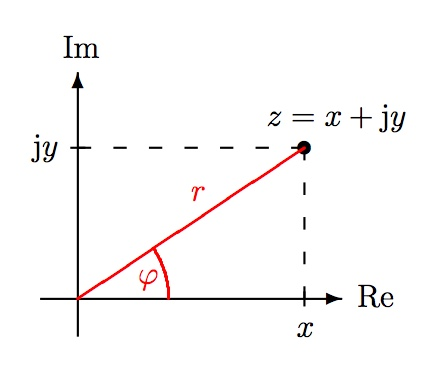
\includegraphics[width=3in]{kap6/komplexezahlen4}

		\begin{Bemerkung}
		Erinnerung\\
		\end{Bemerkung}

		Zusammenhang zwischen den Koordinaten $P(x,y)$ und $P(r,\varphi)$ :\\

		$
		\begin{pmatrix}
		x=r*cos(\varphi)\\
		\\
		y=r*sin(\varphi)
		\end{pmatrix}
		$
		bzw.
		$
		\begin{pmatrix}
		r= \sqrt{x^2+y^2}\\
		\\
		tan(\varphi) = \frac{y}{x}
		\end{pmatrix}
		$
		\\
		\\

		\begin{Bemerkung}
		Bemerkung\\
		\end{Bemerkung}

		Der Zusammenhang zwischen dem Quotienten $\frac{x}{y}$ und dem Winkel $\varphi \in [0,2\pi)$ eindeutig, da die Tangensfunktion -periodisch ist.\\
		Damit erhält man die \textbf{trigonometrische Darstellung} :\\

		$z=x+j*y =r*cos(\varphi)+j*r*sin(\varphi) \Rightarrow z=r(cos(\varphi)+j*sin(\varphi))$\\

		Dieser Ausdruck von $z$ wird im Folgenden sehr h"aufig auftreten. Deshalb wird daf"ur die Abk"urzung\\
		\\
		$e^{j\varphi} =cos(\varphi)+j*sin(\varphi)$\\
		\\
		ein.
		Somit ergibt sich schließlich eine sehr kompakte Darstellung, die sogenannte \textbf{Exponentialdarstellung} einer komplexen Zahl:\\\\
		$z=  {r(cos(\varphi)+r*j*sin(\varphi))}=r*e^{j\varphi}$

		\begin{Bemerkung}
		Zusammenfassung\\
		\end{Bemerkung}

		Eine komplexe Zahl l"asst sich auf verschiedene Arten darstellen:\\


		\begin{tcolorbox}

		\begin{enumerate}

		\item $z=x+j*y$ (kartesische Darstellung)
		\item $z=(cos(\varphi)+j*sin(\varphi))$ (trigonometrische Darstellung)
		\item $z=r*e^{j\varphi}$ (Exponential-Darstellung)\\

		\end{enumerate}

		\end{tcolorbox}


	\subsection{Umrechnung zwischen den Darstellungen}
